+\documentclass[12pt]{article}
\usepackage[utf8]{inputenc}
\usepackage[pdftex]{graphicx}
\usepackage{graphicx}
\usepackage{geometry}
\usepackage{indentfirst}
\usepackage{setspace}
\usepackage{anysize}
\usepackage{makeidx}
\usepackage[brazil]{babel}
\usepackage{longtable}
\usepackage{multirow} 
\usepackage{hyperref}
\makeindex

\newcommand{\longtableendfoot}{Continuará na próxima página}

\geometry{
verbose,
a4paper,
left = 30mm,
top = 30mm,
right = 20mm,
bottom = 20mm
}

\begin{document}
\begin{titlepage}
% \doublespacing
\centering

\normalfont


\vspace{0.1\textheight}
\vbox{\normalfont{UNB - UNIVERSIDADE DE BRASÍLIA\\CAMPUS GAMA}}
\large{Universidade de Brasília - UnB Gama\\}
\vspace{4cm}


\vbox{\Huge
%Nome do Trabalho
DOCUMENTO DE VISÃO PRELIMINAR

%\ver

\vspace{0.03\textheight}
\hrule }

\vbox{
%Nome da Matéria
Introdução à Jogos Eletrônicos
}
\vspace{0.3\textheight}
%Nomes
\vbox{\scshape
{}
  Game Designer: Paulo Markes
  }
\vspace{0.3cm}
{}
\centering
markes.calado@gmail.com \\
\vspace{0.2\textheight}
Brasília, DF~-~\the\year
\end{titlepage}

\onehalfspacing
\tableofcontents
\pagebreak
\section*{Histórico de versionamento}
\begin{longtable}{|l|l|l|}
\hline
\multicolumn{3}{|c|}{Lista de modificações no GDD}
\\
\hline
Data & Autor & Modificação
\\
\hline
08-05-2015 & Paulo Markes & Versão inicial do GDD
\\
\hline
\\
\hline
\end{longtable}

\newpage
\part*{Características gerais do jogo}
\section{Apresentação do jogo}
\subsection{Objetivo do documento}
O objetivo desse documento é apresentar as características principais do jogo 7 Keys, sua história, mecânicas, a proposta de design entre outras informações importantes para o desenvolvimento do jogo.

\subsection{Objetivo do jogo}     
O principal objetivo do jogo é fugir do santório. O jogador começa na ala de celas e precisa alcançar o térreo. Para finalizar cada fase será necessário encontrar uma chave específica que abra a porta que dá acesso ao andar inferior ou à próxima ala.

\subsection{Características gerais}

O jogo terá uma movimentação semelhante a games do estilo Legend of Zelda a Link to the Past e Fatal Labirinth como principais referências e exemplos os jogos The Binding of Isaac e Metal Gear Solid IV como referência para a mecânica de stealth.

 O jogo baseia-se em dois gêneros: stealth e roguelike. Stealth é um gênero onde o jogador precisa evitar ser notado, utilizando da furtividade para evadir ou elaborar emboscadas para os antagonistas. Jogos do gênero empregam mecânicas como se esconder na sombra, em objetos do cenário, disfarces, e barulhos que podem alertar os inimigos. Roguelike é um subgênero, geralmente de jogos de RPG, que é caracterizado pela geração de mapas aleatórios durante a partida, mapas baseados em tile e permanent death.

Não haverá também coleta de moedas, diamantes ou qualquer referência a acúmulo de material destinado à compra de itens, vidas etc. Todos os itens necessários para avançar no jogo estarão dispostos nas fases.

O jogo não possuirá um contador de pontos pois foi considerado dispensável devido a mecânica do jogo.

\section{Requisitos Tecnológicos}
Para a atividade de desenvolvimento foi estabelecida a utilização das seguintes ferramentas:

\begin{enumerate}
\item Sistema Operacional: Linux Ubuntu 14.04 64-bits

Este SO foi escolhido por ser uma ferramenta open source e de utilização comum para a maioria da equipe de desenvolvimento.

\item APIs para manipulação de arquivos, áudio e gráfica: SDL2/SDL1.2

API padrão da disciplina.

\item Ferramenta de controle de versão: Git

Ferramenta padrão da disciplina.

\item Depurador: Debugger

Por ser o software padrão do Linux Ubuntu, o depurador Debugger, da suite GNU, será utilizado.

\item Editor de texto: Sublime Text 2 

O editor Sublime Text 2 está sendo utilizado, porém será decidido por um novo editor em breve.

\item Linguagem de script: Lua

Linguagem de script padrão da disciplina.

\item Linguagem de programação: C++

Esta linguagem foi escolhida por ser de compreensão comum para a maioria da equipe de desenvolvimento.

\item Compilador: g++

\end{enumerate}

\section{Front End}
Ao iniciar o jogo algumas telas são apresentadas ao jogador. Elas contém informações básicas porém importantes, como a empresa que desenvolveu o jogo e as tecnologias ligadas à ele. 

No caso do jogo proposto nesse documento, desenvolvido pela Mana Team, a primeira tela ao executar o jogo que aparece é a tela que apresenta o logo da equipe (Figura 1), que é também o mascote da empresa, o peixe boi. Em seguida vem a tela que apresenta as tecnologias utilizadas para desenvolver o jogo (Figura 2), como o GIMP, os programas da Adobe entre outros. Por fim, antes da tela do menu inicial, vemos a tela com a classificação indicativa do jogo (Figura 3). Cada tela ficará visível por 3 segundo e após esse período ocorrerá um efeito de \textit{fade out} com duração de 1 segundo seguido de um efeito de \textit{fade in} também de um segundo que introduzirá a tela seguinte. A música do menu será iniciada no instante em que a primeira tela for carregada.
\begin{figure}[h]
    \centering
    \caption{Tela com logo [provisória] da empresa}
     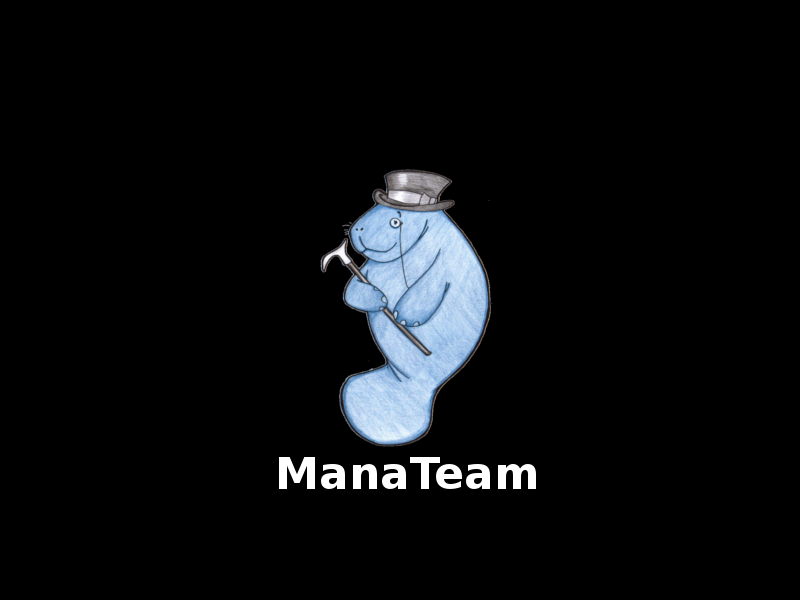
\includegraphics[keepaspectratio=true,scale=0.30]{images/logoMT.png}
\end{figure}
\begin{figure} [!h]
    \centering
    \caption{Tecnologias utilizadas}
    
\includegraphics[keepaspectratio=true,scale=0.30]{images/tecnologias.png}
\end{figure}
\begin{figure}[!h]
    \centering
    \caption{Classificação Indicativa}
    
\includegraphics[keepaspectratio=true,scale=0.30]{images/classificacao_indicativa.png}
\end{figure}

\section{Telas}

\section{Câmera e HUD}
A câmera do jogo é fixa e vista de um ângulo superior inclinado, mais conhecido como \lq\lq visão de pássaro\rq\rq. 

No canto superior esquerdo será apresentado as três barras de dados fundamentais do jogo na seguinte ordem: barra de vida, barra de resistência (stamina) e de sanidade. As barras estão alinhadas a uma imagem do rosto do player que irá variar de acordo com o nível da barra da sanidade.

No canto inferior esquerdo será apresentado os botões de ação do personagem que demonstram os itens que o player poderá utilizar, tanto para ataque quanto para se curar.

\begin{figure}[!h]
    \label{hud}
    \centering
    \caption{Câmera do HUD}
    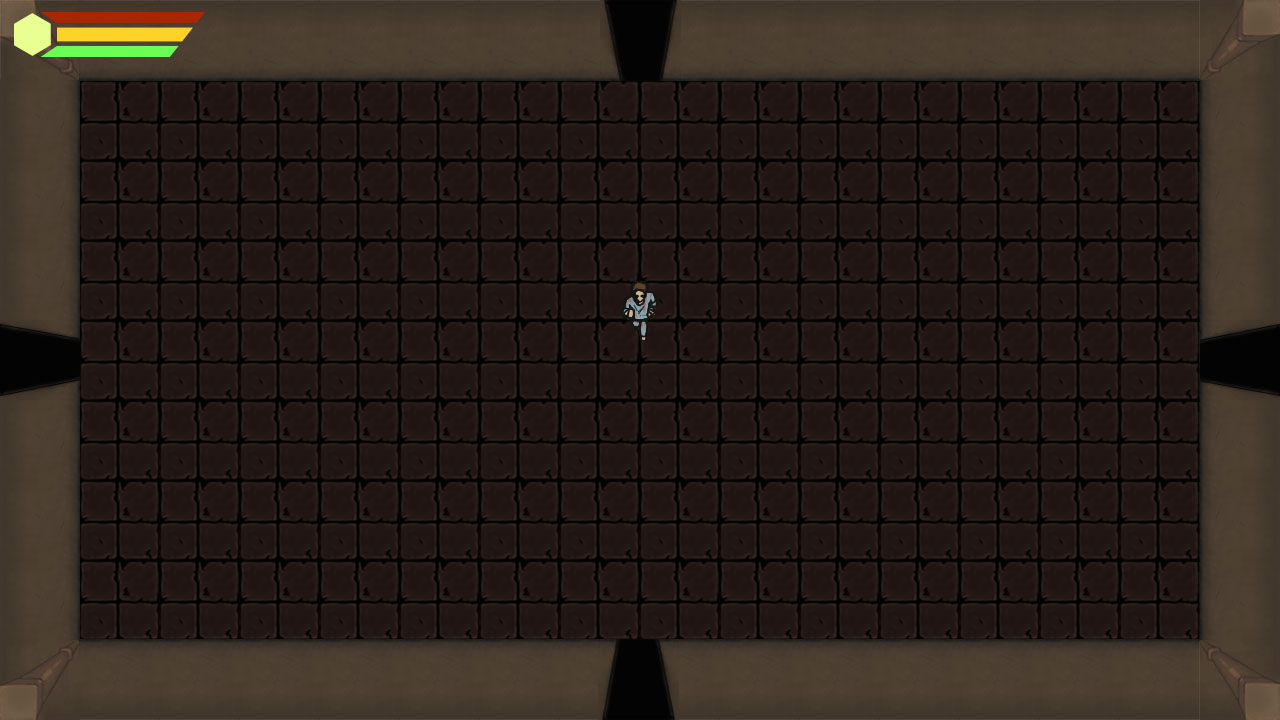
\includegraphics[keepaspectratio=true,scale=0.35]{images/HUD.jpg}
\end{figure}

\section{\label{ctrl} Controles}
O jogador poderá usar como forma de controle para o jogo o teclado do computador ou ainda controles para computadores, mais conhecidos como joysticks. A tabela presente nessa seção apresenta as devidas funcionalidades de ambas as opções dentro do jogo.

\begin{longtable}{|c|c|}
\caption{Controles do jogo}
\\
\hline
\multicolumn{2}{|c|}{Lista de comandos do jogo}
\\
\hline

\includegraphics[scale=0.3]{images/360_Dpad.png}

\includegraphics[scale=0.3]{images/kW.png} 

\includegraphics[scale=0.3]{images/kA.png}

\includegraphics[scale=0.3]{images/kS.png}

\includegraphics[scale=0.3]{images/kD.png}
& Movimentar o personagem na tela
\\
\hline

\includegraphics[scale=0.3]{images/360_RT.png}

\includegraphics[scale=0.3]{images/kShift.png}
 & Correr (na direção selecionada)
\\
\hline

\includegraphics[scale=0.3]{images/360_RB.png}

\includegraphics[scale=0.3]{images/kAlt.png}
& Rolar (na direção selecionada) 
\\
\hline

\includegraphics[scale=0.3]{images/360_LB.png}

\includegraphics[scale=0.3]{images/kCtrl.png}
& Agachar e andar agachado (pressionando algum botão direcional)
\\
\hline

\includegraphics[scale=0.3]{images/360_LT.png}

\includegraphics[scale=0.3]{images/kL.png}
& Ataque com arma secundária
\\
\hline

\includegraphics[scale=0.3]{images/360_A.png}

\includegraphics[scale=0.3]{images/kJ.png}
& Ataque principal (No menu: selecionar opção)
\\
\hline

\includegraphics[scale=0.3]{images/360_B.png}

\includegraphics[scale=0.3]{images/kK.png}
& Interagir com itens (No menu: negar opção)
\\
\hline

\includegraphics[scale=0.3]{images/360_X.png}

\includegraphics[scale=0.3]{images/kQ.png}
& Usar item 
\\
\hline

\includegraphics[scale=0.3]{images/360_Y.png}

\includegraphics[scale=0.3]{images/kE.png}
& Abre a porta especial (ao possuir a chave) 
\\
\hline

\includegraphics[scale=0.3]{images/360_Start.png}

\includegraphics[scale=0.3]{images/kP.png}
& Pausar jogo (acessa o menu de pausa)
\\
\hline
\end{longtable}


\pagebreak
\part*{O mundo do jogo e seus personagens}
\section{A história do jogo}

   Início da 2a Guerra Mundial. A Alemanha invadiu a Polônia, levando a França e o Reino Unido a declarar guerra à Alemanha. O personagem, Edmond Gauthier - um sargento do exército francês - é um homem com um forte senso de honra que lidera bravamente seu exército frente ao inimigo alemão.
   
Em uma missão de resgate na Polônia, Edmond Gauthier e seu exército sofrem uma emboscada, planejada com o principal objetivo de impedi-los de resgatar os reféns judeus que seriam levados ao campo de concentração alemão ainda em construção. Embora a emboscada tenha causado algumas baixas, Edmond consegue alcançar os reféns, porém tarde demais. Ao se aproximar do local, ele percebe que os reféns já haviam sido executados e estavam sendo removidos do caminhão que continha a câmara de gás, uns dos últimos remanescentes da 1ª Guerra Mundial.
   
    Mesmo tendo falhado na missão, o exército francês ataca os alemães, numa espécie de revanche e  aprisiona-os. O superior de Edmond define então que os soldados nazistas aprisionados devem ser fuzilados, o que abala Edmond. Embora seja claro que os nazistas são um mal crescente, o código de honra de Edmond não o permite assassinar homens indefesos, sem a menor chance de revidarem ou sequer se protegerem. No entanto, como a ordem veio de um superior, Edmond é obrigado a obedecer e fuzila os nazistas aprisionados. Após essa missão mal sucedida, e com a crescente ameaça alemã, Edmond resolve voltar ao seu lar na França para se despedir de sua família e os mandarem para a Inglaterra, onde supostamente estariam mais protegidos.
    
    Em 1940, a Alemanha contorna a Linha Magnot - barreira de defesa que cobria toda a fronteira entre a França e a Alemanha, criada pela França após a 1a Guerra Mundial para evitar ataques surpresa e garantir mais tempo de resposta aos franceses em caso de um ataque frontal – vindo pelas densas florestas de Ardenas, único local desprotegido, pois acharam que os tanques alemães não conseguiriam atravessar a floresta. O General Weygand, recentemente nomeado, tomou ações imediatas para conter os alemães. Edmond então é enviado juntamente com o exército francês para conter os alemães. Durante a missão, Dante Chevalier, amigo de Edmond fica sob a mira do fogo inimigo. Edmond, logo parte em sua defesa, abatendo um soldado inimigo de pequeno porte. Ao investigar o corpo do inimigo, Edmond percebe que o soldado era uma criança, de aparentemente menos que 15 anos, o que o deixa perturbado. 
    
    Dois dias depois, ainda tentando conter os alemães, seu esconderijo é atacado por um tanque, desmoronando sobre suas cabeças. Edmond percebe então que Pierre ficou preso nos escombros. Ao tentar resgatar o amigo, acaba notando que o mesmo já se encontrava praticamente sem pulso e desacordado. Edmond decide então, mesmo contra sua vontade, abandonar o amigo e os demais soterrados e foi ao encalço dos alemães.
    
    O exército francês recua enquanto aguarda reforços e, ao receber informes da situação da Europa, descobre que a cidade inglesa onde sua família encontrava-se refugiada foi fortemente bombardeada pelos exércitos alemães. Esse era então o fim para Edmond Gauthier. Nada mais que ele amava lhe restava, além de amargas lembranças dos últimos e turbulentos meses. No entanto, uma missão mais precisava ser cumprida: parar os alemães.
    
    Os alemães, por outro lado, estavam muito fortalecidos e, mesmo com todo o empenho do exército francês e inglês, eles conseguiram avançar adentro do território francês. Edmond e mais alguns oficiais são então aprisionados e torturados em longos interrogatórios. Após obter as informações que necessitavam, os alemães aprisionaram os oficiais no campo de concentração de Bergen- Belsen (ou apenas Belsen) para utilizá-los depois como moeda de troca por oficiais alemães.
    
    Edmond não suporta a pressão causada pelas massivas perdas em sua vida e começa a agir de forma estranha, sendo constantemente atormentado pelas lembranças de seus entes queridos. Sendo considerado como louco, começa a receber uma série de medicações fortes que o deixa 'dopado' por meses a fio. A droga, que ainda estava em experimentação,  é tão forte que começa a afetar as lembranças de Edmond, que lentamente começa a se esquecer de todas as perdas bem como de quem ele próprio é, vivendo em um estágio próximo ao do vegetativo, apenas obedecendo ordens.
    
    Um dia, durante a manutenção do sistema de segurança do campo de concentração, uma pane ocorre no sistema elétrico e a segurança do complexo é comprometida. Praticamente todas as celas do complexo se destravam, o que causa uma tentativa de fuga em massa. Os guardas locais fazem o possível para conter os detentos, enquanto tentam comunicar-se com os campos próximos para solicitar reforços. Edmond, ainda meio sob o efeito dos medicamentos, tenta fugir também, sem atrair a atenção dos guardas. 
    
    Edmond precisará agora utilizar tudo que ainda se lembra para poder sobreviver. Isso significa se esconder nas sombras e atrás de objetos para evitar ser visto pelos guardas. Ou então, quando fugir do guarda não for opção, Edmond precisará eliminá-lo para prosseguir. O complexo em que ele se encontra possui 7 alas divididas em 3 andares, e para fugir ele precisará encontrar chaves específicas que dão acesso aos demais andares/alas até que ele alcance o salão central, que dá acesso aos jardins que por sua vez levam à uma densa floresta, possibilitando uma fuga mais “segura”.
    
    Além de lidar com os guardas, Edmond irá enfrentar outros seres, fantasmas que habitam sua mente. Esses fantasmas possuem características específicas que o relembram fatos importantes de sua vida. Esses fantasmas são, na verdade, suas lembranças de todas as mortes que o impactaram de alguma forma. No entanto, ele precisará lidar com essas lembranças e não só recordá-las como também aceitá-las para conseguir fugir do inferno em que se encontra. Caso contrário, ele será completamente consumido pela insanidade cada vez mais próxima dele, nesse ambiente completamente hostil e cheio de armadilhas, aguardando-o em cada sala. 

\section{Personagem Principal}
Edmond Gauthier, centro da trama do jogo, foi inspirado em soldados franceses que foram presos durante o início da Segunda Guerra Mundial e ficaram em campos de concentração para serem utilizados como moeda de troca. O personagem no início do jogo não consegue se lembrar direito de como ele foi parar naquele sanatório, por estar submetido à uma medicação forte o suficiente para afetar ainda mais a sua mente já deteriorada.

Durante todo o jogo o personagem mistura momentos de lucidez com momentos onde a loucura fala mais alto, que é quando os fantasmas surgem. Nas \textit{cutscenes} isso é mais evidente, onde a mente de Edmond oscila entre as recordações de seu passado, a realidade e a insanidade de sua mente, lutando contra seus fantasmas interiores à medida que tenta recuperar sua memória.

O personagem pode interagir com policiais que tentam conter os prisioneiros em fuga e com loucos que tentam fugir e matam quem encontrar pelo caminho. Ao encontrar um policial, o personagem poderá evitar entrar em seu campo de visão para não ser encontrado. Se o personagem escolher por assassinar o guarda, um fantasma do mesmo surgirá no local para atrapalhar o player, diminuindo sua vida e sanidade gradualmente à medida que permanece próximo à Edmond. Se encontrar um louco, ou o personagem deve tentar fugir o mais rápido possível ou abater o louco, já que o louco irá colocar sua vida em risco tão logo encontre Edmond.

\begin{figure}[h]
    \centering
    \caption{Concept art do Edmond}
     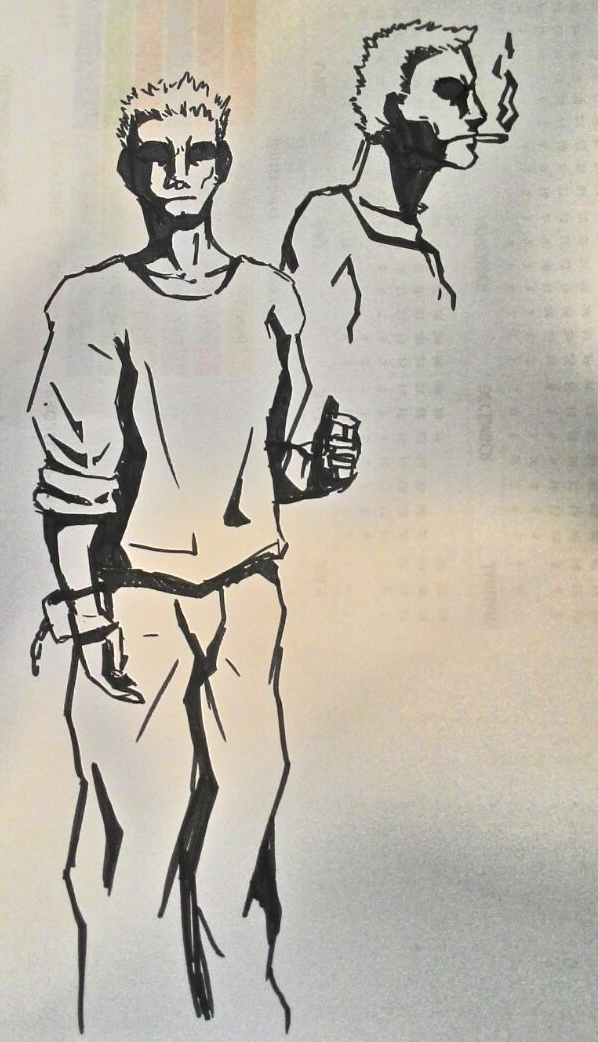
\includegraphics[keepaspectratio=true,scale=0.30]{images/Prev_Ed.png}
\end{figure}

\begin{figure}[h]
    \centering
    \caption{Imagem do Edmond \textit{in game}}
     
\includegraphics[keepaspectratio=true,scale=4]{images/e_ig.png}
\end{figure}
\subsection{Características do personagem}
O personagem terá o tamanho de 2 \textit{tiles} posicionados verticalmente. Cada \textit{tile} possui 40x40px de tamanho. A tela ao todo terá 1280x720px. 

O personagem poderá correr, andar e andar agachado durante o jogo. Ao correr ele se locomoverá a 300px/s, andando ele se locomoverá à 130px/s e ao andar agachado ele se locomoverá a 75px/s.

O personagem poderá interagir com alguns itens durante o jogo, como armas, itens de recuperação de vida e blocos de papéis, todos descritos em seções mais à frente. Para interagir com esses itens, será utilizado os comandos já descritos na seção de controles.

\subsection{Habilidades do personagem}
O personagem possui as habilidades já descritas no tópico anterior: correr, agachar, andar agachado e rolar. Para correr, o personagem terá uma barra de resistência (barra de \textit{Stamina}) que irá determinar um tempo máximo para que o personagem permaneça correndo. Ao reduzir a barra de \textit{stamina} à zero, o personagem será incapaz de permanecer correndo por um tempo, tornando a andar em velocidade normal até que a barra carregue o suficiente para que ele volte a correr.

Todas as habilidades estarão disponíveis ao jogador desde o início do jogo, e o jogador poderá ver como utilizá-las ao acessar  o menu do jogo.

Como o objetivo do jogo será escapar do edifício, não será necessário o uso de transportes para locomoção durante o jogo. 

\subsection{\label{armas}Inventário}
O personagem terá acesso á diversas armas ao longo do jogo, no entanto todas serão de curto alcance. Para utilizá-las, o jogador deverá usar um dos dois tipos de ataque descritos anteriormente. A única arma que usará um controle diferenciado será a arma especial que é a seringa (o seu comando também já foi descrito na seção de controles). 

Os itens serão dispostos no jogo de forma aleatória, de forma que cada item terá uma determinada chance de aparecer de acordo com a fase em que o jogador se encontra. Para trocar de arma, basta que o jogador utilize a opção interagir com itens, descrita no tópico de controles. O jogador só poderá ter uma arma comum e uma arma especial por vez. O mesmo vale para o item de recuperação de vida e sanidade (tópicos que serão melhor detalhados mais a frente). As armas, bem como o dano causado por cada uma delas, será descrito abaixo.

As armas serão: o punho do personagem, faca, garrafa, cacetete e o item especial, seringa.

\subsection{Combate}
O personagem sempre atacará na área de um tile á sua frente. O movimento será sempre o mesmo, o que irá variar é a arma que ele carrega e o dano causado.

Ao ser atacado, o personagem não terá animação que represente o movimento de expressão de dor, mas o personagem irá piscar por alguns segundos e a barra de vida irá diminuir proporcionalmente ao dano, demonstrando que ele foi atacado.

Não existirão combos no jogo.

\section{\label{edmond} Os medidores de saúde do personagem}
\subsection{A vida}
\begin{itemize}
\item Aspectos gerais
\end{itemize}

A vida, aspecto fundamental do personagem, está posicionada no topo da tela, como descrito no HUD, é a primeira das três barras.

O jogo apresentará um item que irá recuperar parte da vida do personagem, o kit  médico. Esse item irá aparecer em localizações e quantidades aleatórias dentro do mapa. O kit médico irá recuperar em 20\% a vida do personagem.

\begin{itemize}
\item Vida e morte no jogo
\end{itemize}

A vida é afetada pelos fantasmas, pelos loucos e pelos policiais dentro do jogo. Como cada um irá afetar a vida do personagem será descrito em sessões mais a frente.

O personagem possui 3 vidas e elas são apresentadas no início de cada fase. Dentro do jogo, ela é representada pela barra vermelha que vai de 0 a 100\%. Ao ter a barra de vida reduzida a 0\% uma vida será descontada. Ao perder a vida, a partida é reiniciada e os itens conseguidos até o momento são mantidos

Ao perder as 3 vidas, a tela de \textit{Game Over} é apresentada e o jogo é reiniciado. Ao reiniciar a partida, o personagem irá perder todos os itens que tiver acumulado ao longo da partida.

\subsection{A \textit{Stamina}}
A barra de \textit{stamina} é a barra que define o quão apto o personagem está para correr. Ela estará posicionada abaixo da barra de vida, como mostrado anteriormente no tópico de Câmera e HUD.

A \textit{stamina}, ou 'resistência', do personagem irá reduzir gradativamente à medida que o personagem permaneça correndo. A barra irá diminuir em aproximadamente 14\% à cada segundo e, após zerada, ficará nesse estado por 3 segundos e então irá recomeçar a recuperar 6\% a cada segundo.

\subsection{A sanidade}
\begin{itemize}
\item O que é
\end{itemize}
A terceira e última barra apresentada no HUD tem importância igual ou até maior que a vida do personagem. Ela é o elemento principal do jogo pois interfere diretamente na mecânica do jogo. 

A barra de sanidade define quão \lq\lq mentalmente são\rq\rq\ o personagem se encontra. Ela pode ser reduzida ao entrar em contato com os fantasmas ou abater um guarda. 

\begin{itemize}
\item Efeitos \textit{in game}
\end{itemize}
Ao ter a sanidade reduzida abaixo dos 40\% a frequência da música mudará e a tela irá começar a tremer com uma frequência proporcional à redução da sanidade. Além disso, os fantasmas existentes no jogo irão se mexer com maior velocidade.

\begin{itemize}
\item Como recuperar a sanidade
\end{itemize}

A sanidade pode ser recuperada de duas formas: perdendo a vida durante o jogo ou recuperando através de um item presente no jogo: a pílula da sanidade.

A  pílula da sanidade recupera 30\% da sanidade do player. No entanto, por se tratar de um medicamento considerado \lq\lq forte\rq\rq o personagem terá uma redução na velocidade de 50\% por 10 segundos. Após esse período, o personagem voltará a ter a velocidade normal.

\pagebreak
\section{\label{characters} Principais Personagens do Mundo do Jogo}
O personagem principal do jogo é o Edmond Gauthier, no entanto, alguns outro personagens também compõe o universo do jogo, apresentados como inimigos do personagem. Essa seção apresenta esses personagens e um pouco de sua relação com o personagem.

Os fantasmas são, na verdade,personagens que só existem dentro da cabeça do Edmond. A função dos fantasmas é fazer com que Edmond perca completamente a sanidade e acabe se tornando mais uma vítima de suas próprias escolhas. No entanto, Edmond deve lutar para consiguir aceitar os fardos adquiridos ao longo da guerra e superar as perdas sofridas no processo.

\subsection{Fantasma dos soldados fuzilados}
Como previamente descrito na história do jogo, Edmond não consegue lidar com algumas mortes, como no caso de alguns soldados que, embora inimigos, não morreram de forma digna, segundo o pensamento do Edmond. 
	
	A forma do personagem tem o objetivo de lembrar o Edmond sobre o significado daquele personagem. Isso justifica os furos que o mesmo tem no corpo, representando os tiros disparados nos soldados fuzilados. 
	
	Esse fantasma aparece para o Edmond na primeira fase para impedi-lo de alcançar o andar inferior.

\subsection{Fantasma do soldado criança}
 O fantasma referente ao soldado criança se parece um pouco com o fantasma dos soldados fuzilados pois esse também era um soldado inimigo. Edmond também é perturbado pelo fato de ter matado a sangue frio uma criança, mesmo que o tenha feito para garantir a segurança de seu amigo e aliado de guerra. [INSERIR AQUI IMAGEM E DESCRIÇÃO DO FANTASMA IN GAME E VERSÃO CUTSCENE]
 
 Esse fantasma irá aparecer na segunda fase do jogo. Por representar o fantasma de uma criança, esse fantasma irá tentar pregar "peças" no jogador, como rindo em momentos aleatórios da fase, e  aparecendo em momentos diferentes do primeiro fantasma.
 
\subsection{Fantasma dos reféns da câmara de gás}
Esse fantasma, que tem a base do seu corpo formada por gás, representa uma das maiores falhas de Edmond durante a guerra, a falha na missão de resgate dos reféns judeus na Polônia, como já relatado na história do jogo.

A pressão causada por essa lembrança na mente de Edmond é tão forte ou até maior que as outras e isso impacta diretamente na relação dele com o fantasma e com a fase em si. O fantasma estará presente em mais momentos da fase, interagindo direta e indiretamente com o Edmond com maior frequência que os anteriores. Esse fantasma estará na terceira fase do jogo.

\subsection{A Cecille}

A única NPC (\textit{Non playable character}) presente no jogo, irá aparecer na última frase e irá ter apenas uma interação com o personagem, porém ela será fundamental para mostrar que o fim se aproxima. 

Cecille é uma das detentas do campo de concentração/ manicômio que aproveitou o caos gerado no local pra poder fugir. Ela costumava interagir, de forma tímida, com Edmond durante os horários de refeição dos detentos. Tem uma admiração muito forte por ele e  é capaz de fazer qualquer coisa para protegê-lo. 

Ao vê-lo durante a última fase, ela irá entregar uma seringa com sonífero para Edmond, irá alertá-lo que aquela arma será útil no futuro e irá avisar que a saída está próxima.

A seringa, diferente dos itens normais, é considerada uma arma especial, que não anula a arma principal, mas acaba depois de um ataque.
\pagebreak
\part*{Mecânicas Universais do jogo}
\section{Mecânica}
 O jogo se inicia no último andar do campo de concentração de Belsen.O mapa será como o mostrado na figura \ref{hud}. O personagem estará em uma ala aberta no início do jogo. O objetivo de cada fase é procurar a chave que dá acesso á fase seguinte. Essa chave está em algum local aleatório das salas que são geradas de forma aleatória.O formato da chave pode mudar de uma fase para outra, mas será sempre um objeto que destrava uma porta específica em alguma sala para a fase seguinte. Toda vez que o jogador perder (for pego por um guarda ou for abatido) o mapa é carregado novamente. Na história, a justificativa para essa mecânica é que a cada vez que ele é capturado e consegue fugir novamente, ele pensa em como conseguir fugir se a estrutura for diferente.

Na seção \ref{ctrl} foi mostrado todas as formas de controlar o personagem dentro do jogo. Nos tópicos dentro dessa seção será detalhado como se dará essa interação entre o personagem e os itens.

\section{Movimentando os itens}
Os itens serão gerados de forma aleatória nas salas, logo, ocasionalmente, o jogador poderá encontrar uma cadeira ou mesa na frente da porta. Nesses casos, ao utilizar a opção de interagir com itens ('B' no joystick do XBOX 360 / K no teclado) o personagem poderá mover os objetos em cena.

\section{Itens coletáveis}
Alguns itens serão coletáveis pelo personagem, para coletá-los é só seguir os comandos descritos na seção \ref{ctrl} (Controles). Os itens serão os itens de saúde descritos na seção \ref{edmond}, a pílula e o kit médico, no caso.

Além desses itens, o personagem poderá coletar armas que estão descritos no tópico \ref{armas} e papéis que estarão espalhados pelo chão das fases. Esses papéis poderão conter detalhes de suas experiências anteriores e durante o seu aprisionamento.

\subsection{\label{colecionaveis}{Itens colecionáveis}}
Os papéis que estão espalhados por todas as fases podem conter trechos da história de Edomond e ao ser encontrado, o personagem visualiza ele na tela e então ele é liberado na seção de extras. 

\section{Inimigos}
\subsection{Guardas}

Os guardas, inimigos mais frequentes do jogo, estarão presentes no jogo desde a primeira fase e são sub-dividos em três tipos, que serão descritos nos próximos itens. São os únicos inimigos capazes de retirar uma vida do personagem, independentemente da quantidade de vida que o mesmo possua.

Os guardas estarão munidos de uma lanterna, para investigar as salas em busca de fugitivos. Uma vez que o policial avistar o personagem principal, ele emitirá um grito de ordem e, se o personagem não abater o policial em até dois segundos, o jogo congelará e uma animação mostrando mais policiais chegando para aprisionar o personagem terá início. A tela apaga e, se o personagem ainda tiver alguma vida, a partida é reiniciada e uma vida é descontada do personagem. Caso o personagem tenha perdido a última vida, a tela de \textit{Game Over} aparece.

\subsubsection*{Guarda medroso}

O guarda do tipo "medroso" é o guarda mais fácil de se esquivar, pois ele fica parado onde aparecer e apenas gira ao redor do próprio eixo, sem coragem de desbravar o cenário atrás dos fugitivos. No entanto, se ele avistar o personagem, ele alerta os demais para juntos pegarem um mero prisioneiro.

\subsubsection*{Guarda acomodado}

O guarda acomodado finge que está trabalhando, andando de um lado para o outro, mas sempre dentro de um eixo pré-determinado (Y ou X). Faz o mesmo que o anterior ao encontrar o personagem.

\subsubsection*{Guarda pertubado}

Completamente assustado com a atual situação, esse guarda anda em todas as direções, completamente sem rumo, em busca de algum fugitivo perdido pelas salas. Além disso, ele anda mais rápido também.

\subsection{Loucos}

Os loucos são.... bem.... loucos. Seres completamente aleatórios que irão te atacar sem te avistarem. São agressivos e barulhentos, o que também pode ser um problema. 

Diferente do policial que ao encontrar o personagem tira uma vida inteira, o louco, ao atacá-lo, tira um percentual da vida. A cada golpe o louco remove 25\% da vida do personagem. Podem estar em qualquer lugar da sala, inclusive escondidos ou disfarçados de itens.

\subsection{Fantasmas}
Os fantasmas são divididos em dois grupos, os fantasmas comuns e os especiais, conforme descrito na seção \ref{characters}. Os fantasmas comuns surgirão sempre que o jogador abater um guarda durante o jogo. 

O fantasma surgirá então na posição que o guarda se encontrava antes de ser abatido. Ele irá vagar aleatoriamente pela sala, ocasionalemnte vindo ao encontro do player. 

Ao permanecer próximo ao jogador, o fantasma reduz a vida do personagem em 10\% a cada contato e 15\% da barra de sanidade.

A medida que a barra de sanidade for reduzida, a velocidade do fantasma é incrementada, o que pode aumentar o número de contatos com o player, reduzindo ainda mais a vida e a sanidade do mesmo, forçando o player a fugir daquela sala o mais rápido possível.

\section{Níveis}

\section{Progresso do Jogo}

\pagebreak
\part*{Sonoplastia}

\section{Músicas e Efeitos Sonoros}

As músicas e os efeitos sonoros serão essenciais para a imersão no jogo, em conjunto com a arte. Elas possuem o objetivo de causar no jogador um sentimento de tensão constante, com melodias mais lentas e efeitos sonoros específicos de cada fase, que são vinculados à partes da história contida em cada fase. 

Nessa seção estão descritos todos os arquivos de áudio que serão utilizados no jogo. Cada fase terá uma música específica e um conjunto de efeitos sonoros padrões para todas as fases, além dos efeitos específicos, descritos no tópico \ref{efx}. 
\subsection{Músicas}
\begin{list}{}{}
\item\textbf{Nome:} abertura.ogg;

\textbf{Quando será utilizado:} música de abertura do jogo, será iniciada quando o jogo começar a ser executado até o jogador sair do menu principal; \\

\item\textbf{Nome:} fase1.ogg;

\textbf{Quando será utilizado:} será executada durante toda a fase 1; \\

\item\textbf{Nome:} fase2.ogg;

\textbf{Quando será utilizado:} será executada durante toda a fase 2; \\

\item\textbf{Nome:} fase3.ogg;

\textbf{Quando será utilizado:} será executada durante toda a fase 3; \\

\item\textbf{Nome:} fase4.ogg;

\textbf{Quando será utilizado:} será executada durante toda a fase 4; \\

\item\textbf{Nome:} fase5.ogg;

\textbf{Quando será utilizado:} será executada durante toda a fase 5; \\

\item\textbf{Nome:} ending.ogg;

\textbf{Quando será utilizado:} será executada ao final do jogo, quando o jogador terminar o jogo; \\


\end{list}
\subsection{\label{efx}Efeitos sonoros gerais}
\begin{list}{}{}
\item\textbf{Nome: } navegacaomenu.ogg;

\textbf{Descrição: } som curto de navegação nos menus;

\textbf{Quando será utilizado: } som de navegação no menu in game e no menu principal. Será acionado toda vez que o jogador selecionar um dos itens do menu; \\


\item\textbf{Nome:} key.ogg;

\textbf{Descrição:} som semelhante a um badalar de um sino;

\textbf{Quando será utilizado:} sempre que o jogador pegar a chave em alguma fase; \\

\item\textbf{Nome:} finalFase.ogg;

\textbf{Descrição:} toque curto de sanfona;

\textbf{Quando será utilizado:} som executado ao final da fase, quando o jogador inserir a chave na porta e passar para a próxima fase; \\

\item\textbf{Nome:} gritoGuarda.ogg;

\textbf{Descrição:} um grito em alemão com voz masculina;

\textbf{Quando será utilizado:} ao avistar o jogador, o guarda irá se espantar e gritar, chamando a atenção do jogador;  \\

\item\textbf{Nome:} danger.ogg;

\textbf{Descrição:} som curto demonstrando perigo;

\textbf{Quando será utilizado:} ao avistar o jogador, o guarda irá gritar para o jogador e esse som será executado junto ao grito, indicando o espanto do guarda e avisando o player do perigo iminente; \\

\item\textbf{Nome:} capturado.ogg;

\textbf{Descrição:} som de fade out sinalizando a derrota do personagem;

\textbf{Quando será utilizado:} Quando o player for capturado pelos guardas da fase; \\

\item\textbf{Nome:} gameover.ogg;

\textbf{Descrição:} som grave com fade out indicando que a partida acabou;

\textbf{Quando será utilizado:} Quando o player perder todas as vidas e a tela de game over aparecer; \\


\item\textbf{Nome:} correndo.ogg;

\textbf{Descrição:} som de uma pessoa correndo;

\textbf{Quando será utilizado:} toda vez que o personagem correr; \\

\item\textbf{Nome:} ataquesoco.ogg;

\textbf{Descrição:} som abafado representando um soco;

\textbf{Quando será utilizado:} toda vez que o personagem desferir um soco em alguém; \\

\item\textbf{Nome:} ataquefaca.ogg;

\textbf{Descrição:} som de algo como vísceras se rasgando;

\textbf{Quando será utilizado:} toda vez que o personagem desferir uma facada em alguém; \\

\item\textbf{Nome:} ataquegarrafa.ogg;

\textbf{Descrição:} som de vidro sendo quebrado;

\textbf{Quando será utilizado:} toda vez que o personagem desferir uma garrafada em alguém;  \\
\end{list}

\subsection{\label{efxF}Efeitos sonoros específicos de cada fase}
\begin{list}{}{}
\item\textbf{\textit{Fase 1}}
\item\textbf{Nome:} alarme.ogg;

\textbf{Descrição:} som de um alarme de presídio;

\textbf{Quando será utilizado:} No início da fase, durante 15 segundos \\

\item\textbf{Nome:} gritoKill.ogg;

\textbf{Descrição:} alemão dando grito de ordem;

\textbf{Quando será utilizado:} Em momentos aleatórios, juntamente com o efeito descrito a seguir; \\

\item\textbf{Nome:} rifleAtirando.ogg;

\textbf{Descrição:} som de metralhadora atirando;

\textbf{Quando será utilizado:} em momentos aleatórios, o jogador ouvirá um grito de ordem em alemão e logo em seguida o som de metralhadora; \\

\item\textbf{\textit{Fase 2}}
\item\textbf{Nome:} criancasRindo.ogg;

\textbf{Descrição:} som de crianças rindo;

\textbf{Quando será utilizado:} Em momentos aleatórios, o jogador escutará o som de crianças sorrindo, que o lembrará do episódio com o soldado criança; \\

\item\textbf{\textit{Fase 3}}
\item\textbf{Nome:} gas.ogg;

\textbf{Descrição:} som de gás escapando;

\textbf{Quando será utilizado:} em momentos aleatórios da fase, o personagem irá ver a sala em que se encontra se encher de gás e ouvirá o barulho do gás escapando;  \\

\item\textbf{Nome:} gritoGas.ogg;

\textbf{Descrição:} som de gritos de pessoas agonizando;

\textbf{Quando será utilizado:} em conjunto com o som do gás escapando, o personagem escutará gritos de agonia que lembrará o personagem das pessoas que morreram na câmara de gás; \\

\textbf{\textit{Fase 4}}
\item\textbf{Nome:} explosão.ogg;

\textbf{Descrição:} som de explosão;

\textbf{Quando será utilizado:} em momentos aleatórios da fase, o personagem escutará o som de uma explosão seguido do efeito descrito a seguir; \\

\item\textbf{Nome:} desmoronamento.ogg;

\textbf{Descrição:} som de um construto sendo desmoronado;

\textbf{Quando será utilizado:} em conjunto com o efeito sonoro descrito anteriormente; \\

\textbf{\textit{Fase 5}}
\item\textbf{Nome:} gritoEsposa.ogg;

\textbf{Descrição:} grito de agonia feminino;

\textbf{Quando será utilizado:} Em momentos aleatórios para referenciar a esposa de Edmond que morreu em uma explosão na Itália; \\

\end{list}
\end{document}